\documentclass[a4paper]{article}

%% Language and font encodings
\usepackage[english]{babel}
\usepackage[utf8x]{inputenc}
\usepackage[T1]{fontenc}

%% Sets page size and margins
\usepackage[a4paper,top=3cm,bottom=2cm,left=3cm,right=3cm,marginparwidth=1.75cm]{geometry}

%% Useful packages
\usepackage{amsmath}
\usepackage{graphicx}
\usepackage[colorinlistoftodos]{todonotes}
\usepackage[colorlinks=true, allcolors=blue]{hyperref}

\title{An angle of flame cone - Bunsen Burner}
\author{Jakub Keciek}

\begin{document}
\maketitle
\section{Introduction}

The purpose of this simulation is to show how cone angle is changing reference to pressure and temperature of burning mixture. Assumptions: flame speed is constans (we can change it manually in program), calculations are made for 1 mole per second expense, nozzle of burner is 1 cm diameter.

\section{Mathematic model}

When burning speed is known we get simple analitycal formula which depends on nozzle diameter $d_l$, flame speed $s_l$, pressure $p$, mole expense $n$ and temperature $T$:

\[\beta = arcsin(\frac{s_l*p*\pi*(\frac{d_l}{2})^2}{n*R*T})\]
\section{Results and conclusions}

Calculations were made for temperatures from 273 to 773 K, for pressure from 1 to 5 bars and for methane-air mixture flame speed 4.1 cm/s.


\begin{figure}[!h]
\centering
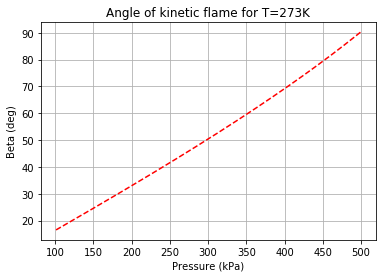
\includegraphics[scale=0.5]{1.png}
\end{figure}

Calculations for T=273K temperature.
\begin{figure}[!h]
\centering
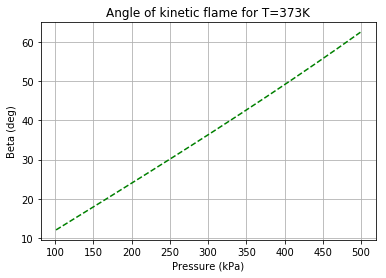
\includegraphics[scale=0.5]{2.png}
\end{figure}

Calculations for T=373K temperature.
\begin{figure}[!h]
\centering
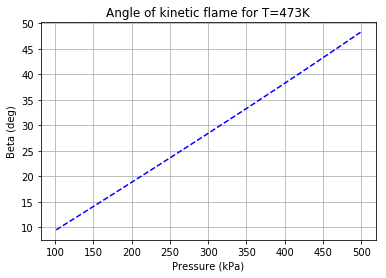
\includegraphics[scale=0.5]{3.png}
\end{figure}

Calculations for T=473K temperature.
\begin{figure}[!h]
\centering
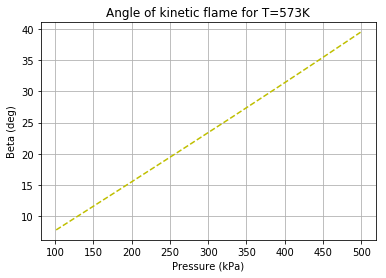
\includegraphics[scale=0.5]{4.png}
\end{figure}

Calculations for T=573K temperature.
\begin{figure}[!h]
\centering
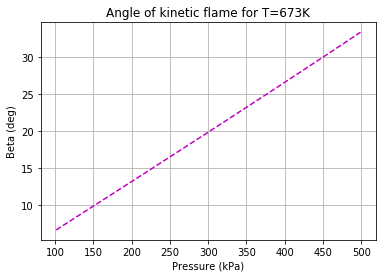
\includegraphics[scale=0.5]{5.png}
\end{figure}

Calculations for T=673K temperature.
\begin{figure}[!h]
\centering
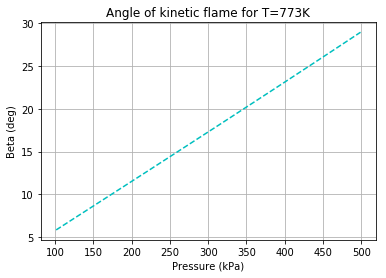
\includegraphics[scale=0.5]{6.png}
\end{figure}

Calculations for T=773K temperature.

As you can see characteristics are nearly linear and the temperature is higher the angle is lower for the same pressure. It can have coincidence with hardly simplified model of calculations.

\section{Bibliography}

Webpages and books used to make project and report:

\url{http://www.plan-rozwoju.pcz.pl/wyklady/kotowicz/W1.pdf}

\url{https://matplotlib.org/users/pyplot_tutorial.html}

\url{https://matplotlib.org/examples/pylab_examples/simple_plot.html}

\url{http://www.cantera.org/docs/sphinx/html/cython/tutorial.html}

\url{http://www.cantera.org/docs/sphinx/html/cython/constants.html}

\url{http://www.cantera.org/docs/sphinx/html/cython/thermo.html}

\url{http://www.cantera.org/docs/sphinx/html/cython/examples/onedim_flamespeed_sensitivity.html}

\url{http://www.cantera.org/docs/sphinx/html/cython/onedim.html}

Marian Gieras "Spalanie. Wybrane zagadnienia w zadaniach"

\end{document}